\documentclass[uplatex,dvipdfmx,11pt]{jsarticle}
\usepackage{amsmath,amssymb,amsthm,mathtools}
\usepackage{geometry}
\usepackage{bm}
\usepackage{graphicx}
\usepackage{tikz}
\usetikzlibrary{arrows.meta,positioning}
\usepackage[unicode]{hyperref}
\providecommand{\cInv}{\cos^{-1}}
\providecommand{\E}{\mathrm{E}}
\providecommand{\V}{\mathrm{V}}
\providecommand{\Cov}{\mathrm{Cov}}
\geometry{margin=24mm}

\begin{document}
\begin{center}
{\LARGE\bfseries MORTRA 検証済み解答\par}
\vspace{1mm}
{\small 分野：解析・幾何\qquad 問題・厳密解・図・証明経路・講評}
\end{center}
\vspace{1mm}
\hrule
\vspace{5mm}

\section*{問題}
原点を $O$，曲線 $P$ を
\[
  P:\ y = x^2
\]
とする.\\
$P$ を $O$ を中心として角 $\theta$ だけ回転させてできる曲線を $Q$ とし，\\
曲線 $P$ と $Q$ で囲まれた領域を $x$ 軸周りに回転させた体積を $V(\theta)$とする.
\[
  \lim_{\theta \to 0} \theta^5 V(\theta)
\]
 の値を求めよ.

\section*{答え}
\(\text{両側極限は存在しない。}\quad \lim_{\theta\to0^+}\theta^5V(\theta)=\frac{128 \pi}{15},\quad \lim_{\theta\to0^-}\theta^5V(\theta)=- \frac{128 \pi}{15}.\)

\section*{解答}
\textbf{1.} 曲線を \(y=ax^2\) と書く。この問題では \(a=1\) である。まず \(\theta>0\) とし、半角変数 \(t=\tan(\theta/2)>0\) によって回転行列を有理化する。

\textbf{2.} 回転前の点を \((u,au^2)\) とすると、交点式は \[-\frac{2tu(atu-1)(2a^2u^2+2atu+t^2+1)}{(1+t^2)^2}=0.\] 二次因子の判別式は負なので、境界の交点は \(O\) と \(R=(-1/(at),1/(at^2))\) だけである。

\textbf{3.} 囲まれた領域を \(\Omega_{\theta}\) とする。これは \(x\) 軸より上にあるから、円環法とグリーンの公式により、境界を時計回りに一周して \[V(\theta)=\pi\oint_{\partial\Omega_{\theta}}^{\rm clockwise}y^2\,dx\] と書ける。固定放物線を \(O\to R\)、回転放物線を \(R\to O\) と進む。

\textbf{4.} 固定放物線上の積分と回転放物線上の積分はそれぞれ \[-\frac1{5a^3t^5},\qquad \frac{8t^2+7}{15a^3t^5(1+t^2)}.\] 従って \[V(\theta)=\frac{\pi(5t^2+4)}{15a^3t^5(1+t^2)}.\]

\textbf{5.} \(\theta/t\to2\) より右極限は \(\frac{128 \pi}{15}\) である。負の角の図形は正の角の図形を \(y\) 軸について反転したものなので \(V(-\theta)=V(\theta)\) であり、左極限は \(- \frac{128 \pi}{15}\) となる。従って両側極限は存在しない。

\clearpage

\section*{一手ずつ見る図解}

\subsection*{1. 回転を半角変数へ移す}

回転行列を半角変数 t の有理式にし、微小角で発散する座標を有限尺度へ移します。

\[
t=\tan(\theta/2),\quad X=atx,\quad Y=at^2y
\]

\begin{center}

\begin{tikzpicture}[scale=5.454545,line cap=round,line join=round]
\path[use as bounding box] (-1.18000000,-0.12000000) rectangle (0.30000000,1.20000000);
\draw[->,black!35] (-1.18000000,0)--(0.30000000,0);
\draw[->,black!35] (0,-0.12000000)--(0,1.20000000);
\draw[draw=cyan!65!black,line width=.7pt] (-1.05000000,1.10250000) -- (-1.04016667,1.08194669) -- (-1.03033333,1.06158678) -- (-1.02050000,1.04142025) -- (-1.01066667,1.02144711) -- (-1.00083333,1.00166736) -- (-0.99100000,0.98208100) -- (-0.98116667,0.96268803) -- (-0.97133333,0.94348844) -- (-0.96150000,0.92448225) -- (-0.95166667,0.90566944) -- (-0.94183333,0.88705003) -- (-0.93200000,0.86862400) -- (-0.92216667,0.85039136) -- (-0.91233333,0.83235211) -- (-0.90250000,0.81450625) -- (-0.89266667,0.79685378) -- (-0.88283333,0.77939469) -- (-0.87300000,0.76212900) -- (-0.86316667,0.74505669) -- (-0.85333333,0.72817778) -- (-0.84350000,0.71149225) -- (-0.83366667,0.69500011) -- (-0.82383333,0.67870136) -- (-0.81400000,0.66259600) -- (-0.80416667,0.64668403) -- (-0.79433333,0.63096544) -- (-0.78450000,0.61544025) -- (-0.77466667,0.60010844) -- (-0.76483333,0.58497003) -- (-0.75500000,0.57002500) -- (-0.74516667,0.55527336) -- (-0.73533333,0.54071511) -- (-0.72550000,0.52635025) -- (-0.71566667,0.51217878) -- (-0.70583333,0.49820069) -- (-0.69600000,0.48441600) -- (-0.68616667,0.47082469) -- (-0.67633333,0.45742678) -- (-0.66650000,0.44422225) -- (-0.65666667,0.43121111) -- (-0.64683333,0.41839336) -- (-0.63700000,0.40576900) -- (-0.62716667,0.39333803) -- (-0.61733333,0.38110044) -- (-0.60750000,0.36905625) -- (-0.59766667,0.35720544) -- (-0.58783333,0.34554803) -- (-0.57800000,0.33408400) -- (-0.56816667,0.32281336) -- (-0.55833333,0.31173611) -- (-0.54850000,0.30085225) -- (-0.53866667,0.29016178) -- (-0.52883333,0.27966469) -- (-0.51900000,0.26936100) -- (-0.50916667,0.25925069) -- (-0.49933333,0.24933378) -- (-0.48950000,0.23961025) -- (-0.47966667,0.23008011) -- (-0.46983333,0.22074336) -- (-0.46000000,0.21160000) -- (-0.45016667,0.20265003) -- (-0.44033333,0.19389344) -- (-0.43050000,0.18533025) -- (-0.42066667,0.17696044) -- (-0.41083333,0.16878403) -- (-0.40100000,0.16080100) -- (-0.39116667,0.15301136) -- (-0.38133333,0.14541511) -- (-0.37150000,0.13801225) -- (-0.36166667,0.13080278) -- (-0.35183333,0.12378669) -- (-0.34200000,0.11696400) -- (-0.33216667,0.11033469) -- (-0.32233333,0.10389878) -- (-0.31250000,0.09765625) -- (-0.30266667,0.09160711) -- (-0.29283333,0.08575136) -- (-0.28300000,0.08008900) -- (-0.27316667,0.07462003) -- (-0.26333333,0.06934444) -- (-0.25350000,0.06426225) -- (-0.24366667,0.05937344) -- (-0.23383333,0.05467803) -- (-0.22400000,0.05017600) -- (-0.21416667,0.04586736) -- (-0.20433333,0.04175211) -- (-0.19450000,0.03783025) -- (-0.18466667,0.03410178) -- (-0.17483333,0.03056669) -- (-0.16500000,0.02722500) -- (-0.15516667,0.02407669) -- (-0.14533333,0.02112178) -- (-0.13550000,0.01836025) -- (-0.12566667,0.01579211) -- (-0.11583333,0.01341736) -- (-0.10600000,0.01123600) -- (-0.09616667,0.00924803) -- (-0.08633333,0.00745344) -- (-0.07650000,0.00585225) -- (-0.06666667,0.00444444) -- (-0.05683333,0.00323003) -- (-0.04700000,0.00220900) -- (-0.03716667,0.00138136) -- (-0.02733333,0.00074711) -- (-0.01750000,0.00030625) -- (-0.00766667,0.00005878) -- (0.00216667,0.00000469) -- (0.01200000,0.00014400) -- (0.02183333,0.00047669) -- (0.03166667,0.00100278) -- (0.04150000,0.00172225) -- (0.05133333,0.00263511) -- (0.06116667,0.00374136) -- (0.07100000,0.00504100) -- (0.08083333,0.00653403) -- (0.09066667,0.00822044) -- (0.10050000,0.01010025) -- (0.11033333,0.01217344) -- (0.12016667,0.01444003) -- (0.13000000,0.01690000);
\draw[draw=magenta!70!black,line width=.7pt] (0.00000000,0.00000000) -- (0.00767575,0.00058814) -- (0.01508244,0.00130645) -- (0.02222007,0.00215493) -- (0.02908864,0.00313358) -- (0.03568815,0.00424241) -- (0.04201860,0.00548140) -- (0.04807999,0.00685057) -- (0.05387231,0.00834991) -- (0.05939558,0.00997942) -- (0.06464979,0.01173910) -- (0.06963494,0.01362895) -- (0.07435103,0.01564897) -- (0.07879805,0.01779917) -- (0.08297602,0.02007953) -- (0.08688493,0.02249007) -- (0.09052478,0.02503078) -- (0.09389556,0.02770166) -- (0.09699729,0.03050271) -- (0.09982995,0.03343393) -- (0.10239356,0.03649533) -- (0.10468811,0.03968689) -- (0.10671359,0.04300863) -- (0.10847002,0.04646054) -- (0.10995738,0.05004262) -- (0.11117569,0.05375487) -- (0.11212493,0.05759729) -- (0.11280511,0.06156989) -- (0.11321624,0.06567265) -- (0.11335830,0.06990559) -- (0.11323131,0.07426869) -- (0.11283525,0.07876197) -- (0.11217013,0.08338542) -- (0.11123596,0.08813904) -- (0.11003272,0.09302284) -- (0.10856042,0.09803680) -- (0.10681906,0.10318094) -- (0.10480864,0.10845524) -- (0.10252917,0.11385972) -- (0.09998063,0.11939437) -- (0.09716303,0.12505919) -- (0.09407637,0.13085419) -- (0.09072065,0.13677935) -- (0.08709587,0.14283468) -- (0.08320203,0.14902019) -- (0.07903913,0.15533587) -- (0.07460717,0.16178172) -- (0.06990615,0.16835774) -- (0.06493607,0.17506393) -- (0.05969693,0.18190029) -- (0.05418873,0.18886683) -- (0.04841147,0.19596353) -- (0.04236515,0.20319041) -- (0.03604977,0.21054746) -- (0.02946532,0.21803468) -- (0.02261182,0.22565207) -- (0.01548926,0.23339963) -- (0.00809764,0.24127736) -- (0.00043695,0.24928527) -- (-0.00749279,0.25742334) -- (-0.01569159,0.26569159) -- (-0.02415946,0.27409001) -- (-0.03289638,0.28261860) -- (-0.04190236,0.29127736) -- (-0.05117741,0.30006630) -- (-0.06072151,0.30898540) -- (-0.07053468,0.31803468) -- (-0.08061690,0.32721412) -- (-0.09096819,0.33652374) -- (-0.10158853,0.34596353) -- (-0.11247794,0.35553349) -- (-0.12363640,0.36523362) -- (-0.13506393,0.37506393) -- (-0.14676051,0.38502440) -- (-0.15872616,0.39511505) -- (-0.17096087,0.40533587) -- (-0.18346463,0.41568686) -- (-0.19623746,0.42616802) -- (-0.20927935,0.43677935) -- (-0.22259030,0.44752085) -- (-0.23617030,0.45839253) -- (-0.25001937,0.46939437) -- (-0.26413750,0.48052639) -- (-0.27852469,0.49178858) -- (-0.29318094,0.50318094) -- (-0.30810625,0.51470347) -- (-0.32330062,0.52635617) -- (-0.33876404,0.53813904) -- (-0.35449653,0.55005209) -- (-0.37049808,0.56209531) -- (-0.38676869,0.57426869) -- (-0.40330836,0.58657225) -- (-0.42011710,0.59900598) -- (-0.43719489,0.61156989) -- (-0.45454174,0.62426396) -- (-0.47215765,0.63708820) -- (-0.49004262,0.65004262) -- (-0.50819665,0.66312721) -- (-0.52661974,0.67634196) -- (-0.54531189,0.68968689) -- (-0.56427311,0.70316200) -- (-0.58350338,0.71676727) -- (-0.60300271,0.73050271) -- (-0.62277111,0.74436833) -- (-0.64280856,0.75836411) -- (-0.66311507,0.77249007) -- (-0.68369065,0.78674620) -- (-0.70453528,0.80113250) -- (-0.72564897,0.81564897) -- (-0.74703173,0.83029562) -- (-0.76868354,0.84507243) -- (-0.79060442,0.85997942) -- (-0.81279435,0.87501657) -- (-0.83525335,0.89018390) -- (-0.85798140,0.90548140) -- (-0.88097852,0.92090907) -- (-0.90424469,0.93646692) -- (-0.92777993,0.95215493) -- (-0.95158423,0.96797312) -- (-0.97565758,0.98392147) -- (-1.00000000,1.00000000);
\fill[cyan!65!black] (0.00000000,0.00000000) circle (1.25pt);
\node[font=\scriptsize,anchor=south west,text=cyan!65!black] at (0.00000000,0.00000000) {O};
\end{tikzpicture}

\end{center}

\subsection*{2. 囲まれた領域を確定する}

二次因子の判別式が負なので、二曲線の実交点は O と R だけです。

\[
R=\left(-\frac1{at},\frac1{at^2}\right)
\]

\begin{center}

\begin{tikzpicture}[scale=5.454545,line cap=round,line join=round]
\path[use as bounding box] (-1.18000000,-0.12000000) rectangle (0.30000000,1.20000000);
\draw[->,black!35] (-1.18000000,0)--(0.30000000,0);
\draw[->,black!35] (0,-0.12000000)--(0,1.20000000);
\draw[draw=cyan!65!black,line width=.7pt] (-1.05000000,1.10250000) -- (-1.04016667,1.08194669) -- (-1.03033333,1.06158678) -- (-1.02050000,1.04142025) -- (-1.01066667,1.02144711) -- (-1.00083333,1.00166736) -- (-0.99100000,0.98208100) -- (-0.98116667,0.96268803) -- (-0.97133333,0.94348844) -- (-0.96150000,0.92448225) -- (-0.95166667,0.90566944) -- (-0.94183333,0.88705003) -- (-0.93200000,0.86862400) -- (-0.92216667,0.85039136) -- (-0.91233333,0.83235211) -- (-0.90250000,0.81450625) -- (-0.89266667,0.79685378) -- (-0.88283333,0.77939469) -- (-0.87300000,0.76212900) -- (-0.86316667,0.74505669) -- (-0.85333333,0.72817778) -- (-0.84350000,0.71149225) -- (-0.83366667,0.69500011) -- (-0.82383333,0.67870136) -- (-0.81400000,0.66259600) -- (-0.80416667,0.64668403) -- (-0.79433333,0.63096544) -- (-0.78450000,0.61544025) -- (-0.77466667,0.60010844) -- (-0.76483333,0.58497003) -- (-0.75500000,0.57002500) -- (-0.74516667,0.55527336) -- (-0.73533333,0.54071511) -- (-0.72550000,0.52635025) -- (-0.71566667,0.51217878) -- (-0.70583333,0.49820069) -- (-0.69600000,0.48441600) -- (-0.68616667,0.47082469) -- (-0.67633333,0.45742678) -- (-0.66650000,0.44422225) -- (-0.65666667,0.43121111) -- (-0.64683333,0.41839336) -- (-0.63700000,0.40576900) -- (-0.62716667,0.39333803) -- (-0.61733333,0.38110044) -- (-0.60750000,0.36905625) -- (-0.59766667,0.35720544) -- (-0.58783333,0.34554803) -- (-0.57800000,0.33408400) -- (-0.56816667,0.32281336) -- (-0.55833333,0.31173611) -- (-0.54850000,0.30085225) -- (-0.53866667,0.29016178) -- (-0.52883333,0.27966469) -- (-0.51900000,0.26936100) -- (-0.50916667,0.25925069) -- (-0.49933333,0.24933378) -- (-0.48950000,0.23961025) -- (-0.47966667,0.23008011) -- (-0.46983333,0.22074336) -- (-0.46000000,0.21160000) -- (-0.45016667,0.20265003) -- (-0.44033333,0.19389344) -- (-0.43050000,0.18533025) -- (-0.42066667,0.17696044) -- (-0.41083333,0.16878403) -- (-0.40100000,0.16080100) -- (-0.39116667,0.15301136) -- (-0.38133333,0.14541511) -- (-0.37150000,0.13801225) -- (-0.36166667,0.13080278) -- (-0.35183333,0.12378669) -- (-0.34200000,0.11696400) -- (-0.33216667,0.11033469) -- (-0.32233333,0.10389878) -- (-0.31250000,0.09765625) -- (-0.30266667,0.09160711) -- (-0.29283333,0.08575136) -- (-0.28300000,0.08008900) -- (-0.27316667,0.07462003) -- (-0.26333333,0.06934444) -- (-0.25350000,0.06426225) -- (-0.24366667,0.05937344) -- (-0.23383333,0.05467803) -- (-0.22400000,0.05017600) -- (-0.21416667,0.04586736) -- (-0.20433333,0.04175211) -- (-0.19450000,0.03783025) -- (-0.18466667,0.03410178) -- (-0.17483333,0.03056669) -- (-0.16500000,0.02722500) -- (-0.15516667,0.02407669) -- (-0.14533333,0.02112178) -- (-0.13550000,0.01836025) -- (-0.12566667,0.01579211) -- (-0.11583333,0.01341736) -- (-0.10600000,0.01123600) -- (-0.09616667,0.00924803) -- (-0.08633333,0.00745344) -- (-0.07650000,0.00585225) -- (-0.06666667,0.00444444) -- (-0.05683333,0.00323003) -- (-0.04700000,0.00220900) -- (-0.03716667,0.00138136) -- (-0.02733333,0.00074711) -- (-0.01750000,0.00030625) -- (-0.00766667,0.00005878) -- (0.00216667,0.00000469) -- (0.01200000,0.00014400) -- (0.02183333,0.00047669) -- (0.03166667,0.00100278) -- (0.04150000,0.00172225) -- (0.05133333,0.00263511) -- (0.06116667,0.00374136) -- (0.07100000,0.00504100) -- (0.08083333,0.00653403) -- (0.09066667,0.00822044) -- (0.10050000,0.01010025) -- (0.11033333,0.01217344) -- (0.12016667,0.01444003) -- (0.13000000,0.01690000);
\draw[draw=magenta!70!black,line width=.7pt] (0.00000000,0.00000000) -- (0.00767575,0.00058814) -- (0.01508244,0.00130645) -- (0.02222007,0.00215493) -- (0.02908864,0.00313358) -- (0.03568815,0.00424241) -- (0.04201860,0.00548140) -- (0.04807999,0.00685057) -- (0.05387231,0.00834991) -- (0.05939558,0.00997942) -- (0.06464979,0.01173910) -- (0.06963494,0.01362895) -- (0.07435103,0.01564897) -- (0.07879805,0.01779917) -- (0.08297602,0.02007953) -- (0.08688493,0.02249007) -- (0.09052478,0.02503078) -- (0.09389556,0.02770166) -- (0.09699729,0.03050271) -- (0.09982995,0.03343393) -- (0.10239356,0.03649533) -- (0.10468811,0.03968689) -- (0.10671359,0.04300863) -- (0.10847002,0.04646054) -- (0.10995738,0.05004262) -- (0.11117569,0.05375487) -- (0.11212493,0.05759729) -- (0.11280511,0.06156989) -- (0.11321624,0.06567265) -- (0.11335830,0.06990559) -- (0.11323131,0.07426869) -- (0.11283525,0.07876197) -- (0.11217013,0.08338542) -- (0.11123596,0.08813904) -- (0.11003272,0.09302284) -- (0.10856042,0.09803680) -- (0.10681906,0.10318094) -- (0.10480864,0.10845524) -- (0.10252917,0.11385972) -- (0.09998063,0.11939437) -- (0.09716303,0.12505919) -- (0.09407637,0.13085419) -- (0.09072065,0.13677935) -- (0.08709587,0.14283468) -- (0.08320203,0.14902019) -- (0.07903913,0.15533587) -- (0.07460717,0.16178172) -- (0.06990615,0.16835774) -- (0.06493607,0.17506393) -- (0.05969693,0.18190029) -- (0.05418873,0.18886683) -- (0.04841147,0.19596353) -- (0.04236515,0.20319041) -- (0.03604977,0.21054746) -- (0.02946532,0.21803468) -- (0.02261182,0.22565207) -- (0.01548926,0.23339963) -- (0.00809764,0.24127736) -- (0.00043695,0.24928527) -- (-0.00749279,0.25742334) -- (-0.01569159,0.26569159) -- (-0.02415946,0.27409001) -- (-0.03289638,0.28261860) -- (-0.04190236,0.29127736) -- (-0.05117741,0.30006630) -- (-0.06072151,0.30898540) -- (-0.07053468,0.31803468) -- (-0.08061690,0.32721412) -- (-0.09096819,0.33652374) -- (-0.10158853,0.34596353) -- (-0.11247794,0.35553349) -- (-0.12363640,0.36523362) -- (-0.13506393,0.37506393) -- (-0.14676051,0.38502440) -- (-0.15872616,0.39511505) -- (-0.17096087,0.40533587) -- (-0.18346463,0.41568686) -- (-0.19623746,0.42616802) -- (-0.20927935,0.43677935) -- (-0.22259030,0.44752085) -- (-0.23617030,0.45839253) -- (-0.25001937,0.46939437) -- (-0.26413750,0.48052639) -- (-0.27852469,0.49178858) -- (-0.29318094,0.50318094) -- (-0.30810625,0.51470347) -- (-0.32330062,0.52635617) -- (-0.33876404,0.53813904) -- (-0.35449653,0.55005209) -- (-0.37049808,0.56209531) -- (-0.38676869,0.57426869) -- (-0.40330836,0.58657225) -- (-0.42011710,0.59900598) -- (-0.43719489,0.61156989) -- (-0.45454174,0.62426396) -- (-0.47215765,0.63708820) -- (-0.49004262,0.65004262) -- (-0.50819665,0.66312721) -- (-0.52661974,0.67634196) -- (-0.54531189,0.68968689) -- (-0.56427311,0.70316200) -- (-0.58350338,0.71676727) -- (-0.60300271,0.73050271) -- (-0.62277111,0.74436833) -- (-0.64280856,0.75836411) -- (-0.66311507,0.77249007) -- (-0.68369065,0.78674620) -- (-0.70453528,0.80113250) -- (-0.72564897,0.81564897) -- (-0.74703173,0.83029562) -- (-0.76868354,0.84507243) -- (-0.79060442,0.85997942) -- (-0.81279435,0.87501657) -- (-0.83525335,0.89018390) -- (-0.85798140,0.90548140) -- (-0.88097852,0.92090907) -- (-0.90424469,0.93646692) -- (-0.92777993,0.95215493) -- (-0.95158423,0.96797312) -- (-0.97565758,0.98392147) -- (-1.00000000,1.00000000);
\fill[cyan!65!black] (0.00000000,0.00000000) circle (1.25pt);
\node[font=\scriptsize,anchor=south west,text=cyan!65!black] at (0.00000000,0.00000000) {O};
\fill[black!80] (-1.00000000,1.00000000) circle (1.25pt);
\node[font=\scriptsize,anchor=south west,text=black!80] at (-1.00000000,1.00000000) {R};
\end{tikzpicture}

\end{center}

\subsection*{3. 境界積分で体積を求める}

縦断面の円環面積を境界に沿う一つの積分へまとめ、負の角は対称移動で処理します。

\[
V=\pi\oint_{\partial\Omega}^{\rm clockwise}y^2\,dx
\]

\begin{center}

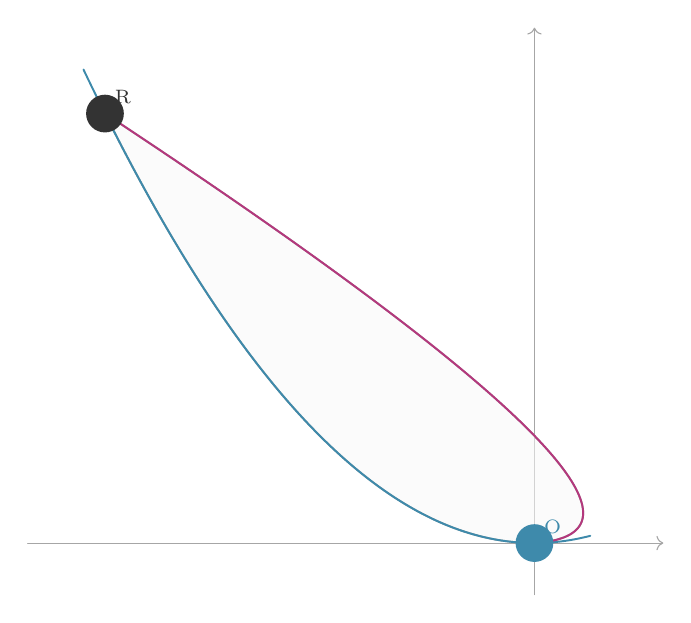
\begin{tikzpicture}[scale=5.454545,line cap=round,line join=round]
\path[use as bounding box] (-1.18000000,-0.12000000) rectangle (0.30000000,1.20000000);
\draw[->,black!35] (-1.18000000,0)--(0.30000000,0);
\draw[->,black!35] (0,-0.12000000)--(0,1.20000000);
\draw[draw=black!38,fill=black!3,line width=.7pt,fill opacity=.55] (0.00000000,0.00000000) -- (-0.01000000,0.00010000) -- (-0.02000000,0.00040000) -- (-0.03000000,0.00090000) -- (-0.04000000,0.00160000) -- (-0.05000000,0.00250000) -- (-0.06000000,0.00360000) -- (-0.07000000,0.00490000) -- (-0.08000000,0.00640000) -- (-0.09000000,0.00810000) -- (-0.10000000,0.01000000) -- (-0.11000000,0.01210000) -- (-0.12000000,0.01440000) -- (-0.13000000,0.01690000) -- (-0.14000000,0.01960000) -- (-0.15000000,0.02250000) -- (-0.16000000,0.02560000) -- (-0.17000000,0.02890000) -- (-0.18000000,0.03240000) -- (-0.19000000,0.03610000) -- (-0.20000000,0.04000000) -- (-0.21000000,0.04410000) -- (-0.22000000,0.04840000) -- (-0.23000000,0.05290000) -- (-0.24000000,0.05760000) -- (-0.25000000,0.06250000) -- (-0.26000000,0.06760000) -- (-0.27000000,0.07290000) -- (-0.28000000,0.07840000) -- (-0.29000000,0.08410000) -- (-0.30000000,0.09000000) -- (-0.31000000,0.09610000) -- (-0.32000000,0.10240000) -- (-0.33000000,0.10890000) -- (-0.34000000,0.11560000) -- (-0.35000000,0.12250000) -- (-0.36000000,0.12960000) -- (-0.37000000,0.13690000) -- (-0.38000000,0.14440000) -- (-0.39000000,0.15210000) -- (-0.40000000,0.16000000) -- (-0.41000000,0.16810000) -- (-0.42000000,0.17640000) -- (-0.43000000,0.18490000) -- (-0.44000000,0.19360000) -- (-0.45000000,0.20250000) -- (-0.46000000,0.21160000) -- (-0.47000000,0.22090000) -- (-0.48000000,0.23040000) -- (-0.49000000,0.24010000) -- (-0.50000000,0.25000000) -- (-0.51000000,0.26010000) -- (-0.52000000,0.27040000) -- (-0.53000000,0.28090000) -- (-0.54000000,0.29160000) -- (-0.55000000,0.30250000) -- (-0.56000000,0.31360000) -- (-0.57000000,0.32490000) -- (-0.58000000,0.33640000) -- (-0.59000000,0.34810000) -- (-0.60000000,0.36000000) -- (-0.61000000,0.37210000) -- (-0.62000000,0.38440000) -- (-0.63000000,0.39690000) -- (-0.64000000,0.40960000) -- (-0.65000000,0.42250000) -- (-0.66000000,0.43560000) -- (-0.67000000,0.44890000) -- (-0.68000000,0.46240000) -- (-0.69000000,0.47610000) -- (-0.70000000,0.49000000) -- (-0.71000000,0.50410000) -- (-0.72000000,0.51840000) -- (-0.73000000,0.53290000) -- (-0.74000000,0.54760000) -- (-0.75000000,0.56250000) -- (-0.76000000,0.57760000) -- (-0.77000000,0.59290000) -- (-0.78000000,0.60840000) -- (-0.79000000,0.62410000) -- (-0.80000000,0.64000000) -- (-0.81000000,0.65610000) -- (-0.82000000,0.67240000) -- (-0.83000000,0.68890000) -- (-0.84000000,0.70560000) -- (-0.85000000,0.72250000) -- (-0.86000000,0.73960000) -- (-0.87000000,0.75690000) -- (-0.88000000,0.77440000) -- (-0.89000000,0.79210000) -- (-0.90000000,0.81000000) -- (-0.91000000,0.82810000) -- (-0.92000000,0.84640000) -- (-0.93000000,0.86490000) -- (-0.94000000,0.88360000) -- (-0.95000000,0.90250000) -- (-0.96000000,0.92160000) -- (-0.97000000,0.94090000) -- (-0.98000000,0.96040000) -- (-0.99000000,0.98010000) -- (-1.00000000,1.00000000) -- (-1.00000000,1.00000000) -- (-0.97565758,0.98392147) -- (-0.95158423,0.96797312) -- (-0.92777993,0.95215493) -- (-0.90424469,0.93646692) -- (-0.88097852,0.92090907) -- (-0.85798140,0.90548140) -- (-0.83525335,0.89018390) -- (-0.81279435,0.87501657) -- (-0.79060442,0.85997942) -- (-0.76868354,0.84507243) -- (-0.74703173,0.83029562) -- (-0.72564897,0.81564897) -- (-0.70453528,0.80113250) -- (-0.68369065,0.78674620) -- (-0.66311507,0.77249007) -- (-0.64280856,0.75836411) -- (-0.62277111,0.74436833) -- (-0.60300271,0.73050271) -- (-0.58350338,0.71676727) -- (-0.56427311,0.70316200) -- (-0.54531189,0.68968689) -- (-0.52661974,0.67634196) -- (-0.50819665,0.66312721) -- (-0.49004262,0.65004262) -- (-0.47215765,0.63708820) -- (-0.45454174,0.62426396) -- (-0.43719489,0.61156989) -- (-0.42011710,0.59900598) -- (-0.40330836,0.58657225) -- (-0.38676869,0.57426869) -- (-0.37049808,0.56209531) -- (-0.35449653,0.55005209) -- (-0.33876404,0.53813904) -- (-0.32330062,0.52635617) -- (-0.30810625,0.51470347) -- (-0.29318094,0.50318094) -- (-0.27852469,0.49178858) -- (-0.26413750,0.48052639) -- (-0.25001937,0.46939437) -- (-0.23617030,0.45839253) -- (-0.22259030,0.44752085) -- (-0.20927935,0.43677935) -- (-0.19623746,0.42616802) -- (-0.18346463,0.41568686) -- (-0.17096087,0.40533587) -- (-0.15872616,0.39511505) -- (-0.14676051,0.38502440) -- (-0.13506393,0.37506393) -- (-0.12363640,0.36523362) -- (-0.11247794,0.35553349) -- (-0.10158853,0.34596353) -- (-0.09096819,0.33652374) -- (-0.08061690,0.32721412) -- (-0.07053468,0.31803468) -- (-0.06072151,0.30898540) -- (-0.05117741,0.30006630) -- (-0.04190236,0.29127736) -- (-0.03289638,0.28261860) -- (-0.02415946,0.27409001) -- (-0.01569159,0.26569159) -- (-0.00749279,0.25742334) -- (0.00043695,0.24928527) -- (0.00809764,0.24127736) -- (0.01548926,0.23339963) -- (0.02261182,0.22565207) -- (0.02946532,0.21803468) -- (0.03604977,0.21054746) -- (0.04236515,0.20319041) -- (0.04841147,0.19596353) -- (0.05418873,0.18886683) -- (0.05969693,0.18190029) -- (0.06493607,0.17506393) -- (0.06990615,0.16835774) -- (0.07460717,0.16178172) -- (0.07903913,0.15533587) -- (0.08320203,0.14902019) -- (0.08709587,0.14283468) -- (0.09072065,0.13677935) -- (0.09407637,0.13085419) -- (0.09716303,0.12505919) -- (0.09998063,0.11939437) -- (0.10252917,0.11385972) -- (0.10480864,0.10845524) -- (0.10681906,0.10318094) -- (0.10856042,0.09803680) -- (0.11003272,0.09302284) -- (0.11123596,0.08813904) -- (0.11217013,0.08338542) -- (0.11283525,0.07876197) -- (0.11323131,0.07426869) -- (0.11335830,0.06990559) -- (0.11321624,0.06567265) -- (0.11280511,0.06156989) -- (0.11212493,0.05759729) -- (0.11117569,0.05375487) -- (0.10995738,0.05004262) -- (0.10847002,0.04646054) -- (0.10671359,0.04300863) -- (0.10468811,0.03968689) -- (0.10239356,0.03649533) -- (0.09982995,0.03343393) -- (0.09699729,0.03050271) -- (0.09389556,0.02770166) -- (0.09052478,0.02503078) -- (0.08688493,0.02249007) -- (0.08297602,0.02007953) -- (0.07879805,0.01779917) -- (0.07435103,0.01564897) -- (0.06963494,0.01362895) -- (0.06464979,0.01173910) -- (0.05939558,0.00997942) -- (0.05387231,0.00834991) -- (0.04807999,0.00685057) -- (0.04201860,0.00548140) -- (0.03568815,0.00424241) -- (0.02908864,0.00313358) -- (0.02222007,0.00215493) -- (0.01508244,0.00130645) -- (0.00767575,0.00058814) -- (0.00000000,0.00000000) -- cycle;
\draw[draw=cyan!65!black,line width=.7pt] (-1.05000000,1.10250000) -- (-1.04016667,1.08194669) -- (-1.03033333,1.06158678) -- (-1.02050000,1.04142025) -- (-1.01066667,1.02144711) -- (-1.00083333,1.00166736) -- (-0.99100000,0.98208100) -- (-0.98116667,0.96268803) -- (-0.97133333,0.94348844) -- (-0.96150000,0.92448225) -- (-0.95166667,0.90566944) -- (-0.94183333,0.88705003) -- (-0.93200000,0.86862400) -- (-0.92216667,0.85039136) -- (-0.91233333,0.83235211) -- (-0.90250000,0.81450625) -- (-0.89266667,0.79685378) -- (-0.88283333,0.77939469) -- (-0.87300000,0.76212900) -- (-0.86316667,0.74505669) -- (-0.85333333,0.72817778) -- (-0.84350000,0.71149225) -- (-0.83366667,0.69500011) -- (-0.82383333,0.67870136) -- (-0.81400000,0.66259600) -- (-0.80416667,0.64668403) -- (-0.79433333,0.63096544) -- (-0.78450000,0.61544025) -- (-0.77466667,0.60010844) -- (-0.76483333,0.58497003) -- (-0.75500000,0.57002500) -- (-0.74516667,0.55527336) -- (-0.73533333,0.54071511) -- (-0.72550000,0.52635025) -- (-0.71566667,0.51217878) -- (-0.70583333,0.49820069) -- (-0.69600000,0.48441600) -- (-0.68616667,0.47082469) -- (-0.67633333,0.45742678) -- (-0.66650000,0.44422225) -- (-0.65666667,0.43121111) -- (-0.64683333,0.41839336) -- (-0.63700000,0.40576900) -- (-0.62716667,0.39333803) -- (-0.61733333,0.38110044) -- (-0.60750000,0.36905625) -- (-0.59766667,0.35720544) -- (-0.58783333,0.34554803) -- (-0.57800000,0.33408400) -- (-0.56816667,0.32281336) -- (-0.55833333,0.31173611) -- (-0.54850000,0.30085225) -- (-0.53866667,0.29016178) -- (-0.52883333,0.27966469) -- (-0.51900000,0.26936100) -- (-0.50916667,0.25925069) -- (-0.49933333,0.24933378) -- (-0.48950000,0.23961025) -- (-0.47966667,0.23008011) -- (-0.46983333,0.22074336) -- (-0.46000000,0.21160000) -- (-0.45016667,0.20265003) -- (-0.44033333,0.19389344) -- (-0.43050000,0.18533025) -- (-0.42066667,0.17696044) -- (-0.41083333,0.16878403) -- (-0.40100000,0.16080100) -- (-0.39116667,0.15301136) -- (-0.38133333,0.14541511) -- (-0.37150000,0.13801225) -- (-0.36166667,0.13080278) -- (-0.35183333,0.12378669) -- (-0.34200000,0.11696400) -- (-0.33216667,0.11033469) -- (-0.32233333,0.10389878) -- (-0.31250000,0.09765625) -- (-0.30266667,0.09160711) -- (-0.29283333,0.08575136) -- (-0.28300000,0.08008900) -- (-0.27316667,0.07462003) -- (-0.26333333,0.06934444) -- (-0.25350000,0.06426225) -- (-0.24366667,0.05937344) -- (-0.23383333,0.05467803) -- (-0.22400000,0.05017600) -- (-0.21416667,0.04586736) -- (-0.20433333,0.04175211) -- (-0.19450000,0.03783025) -- (-0.18466667,0.03410178) -- (-0.17483333,0.03056669) -- (-0.16500000,0.02722500) -- (-0.15516667,0.02407669) -- (-0.14533333,0.02112178) -- (-0.13550000,0.01836025) -- (-0.12566667,0.01579211) -- (-0.11583333,0.01341736) -- (-0.10600000,0.01123600) -- (-0.09616667,0.00924803) -- (-0.08633333,0.00745344) -- (-0.07650000,0.00585225) -- (-0.06666667,0.00444444) -- (-0.05683333,0.00323003) -- (-0.04700000,0.00220900) -- (-0.03716667,0.00138136) -- (-0.02733333,0.00074711) -- (-0.01750000,0.00030625) -- (-0.00766667,0.00005878) -- (0.00216667,0.00000469) -- (0.01200000,0.00014400) -- (0.02183333,0.00047669) -- (0.03166667,0.00100278) -- (0.04150000,0.00172225) -- (0.05133333,0.00263511) -- (0.06116667,0.00374136) -- (0.07100000,0.00504100) -- (0.08083333,0.00653403) -- (0.09066667,0.00822044) -- (0.10050000,0.01010025) -- (0.11033333,0.01217344) -- (0.12016667,0.01444003) -- (0.13000000,0.01690000);
\draw[draw=magenta!70!black,line width=.7pt] (0.00000000,0.00000000) -- (0.00767575,0.00058814) -- (0.01508244,0.00130645) -- (0.02222007,0.00215493) -- (0.02908864,0.00313358) -- (0.03568815,0.00424241) -- (0.04201860,0.00548140) -- (0.04807999,0.00685057) -- (0.05387231,0.00834991) -- (0.05939558,0.00997942) -- (0.06464979,0.01173910) -- (0.06963494,0.01362895) -- (0.07435103,0.01564897) -- (0.07879805,0.01779917) -- (0.08297602,0.02007953) -- (0.08688493,0.02249007) -- (0.09052478,0.02503078) -- (0.09389556,0.02770166) -- (0.09699729,0.03050271) -- (0.09982995,0.03343393) -- (0.10239356,0.03649533) -- (0.10468811,0.03968689) -- (0.10671359,0.04300863) -- (0.10847002,0.04646054) -- (0.10995738,0.05004262) -- (0.11117569,0.05375487) -- (0.11212493,0.05759729) -- (0.11280511,0.06156989) -- (0.11321624,0.06567265) -- (0.11335830,0.06990559) -- (0.11323131,0.07426869) -- (0.11283525,0.07876197) -- (0.11217013,0.08338542) -- (0.11123596,0.08813904) -- (0.11003272,0.09302284) -- (0.10856042,0.09803680) -- (0.10681906,0.10318094) -- (0.10480864,0.10845524) -- (0.10252917,0.11385972) -- (0.09998063,0.11939437) -- (0.09716303,0.12505919) -- (0.09407637,0.13085419) -- (0.09072065,0.13677935) -- (0.08709587,0.14283468) -- (0.08320203,0.14902019) -- (0.07903913,0.15533587) -- (0.07460717,0.16178172) -- (0.06990615,0.16835774) -- (0.06493607,0.17506393) -- (0.05969693,0.18190029) -- (0.05418873,0.18886683) -- (0.04841147,0.19596353) -- (0.04236515,0.20319041) -- (0.03604977,0.21054746) -- (0.02946532,0.21803468) -- (0.02261182,0.22565207) -- (0.01548926,0.23339963) -- (0.00809764,0.24127736) -- (0.00043695,0.24928527) -- (-0.00749279,0.25742334) -- (-0.01569159,0.26569159) -- (-0.02415946,0.27409001) -- (-0.03289638,0.28261860) -- (-0.04190236,0.29127736) -- (-0.05117741,0.30006630) -- (-0.06072151,0.30898540) -- (-0.07053468,0.31803468) -- (-0.08061690,0.32721412) -- (-0.09096819,0.33652374) -- (-0.10158853,0.34596353) -- (-0.11247794,0.35553349) -- (-0.12363640,0.36523362) -- (-0.13506393,0.37506393) -- (-0.14676051,0.38502440) -- (-0.15872616,0.39511505) -- (-0.17096087,0.40533587) -- (-0.18346463,0.41568686) -- (-0.19623746,0.42616802) -- (-0.20927935,0.43677935) -- (-0.22259030,0.44752085) -- (-0.23617030,0.45839253) -- (-0.25001937,0.46939437) -- (-0.26413750,0.48052639) -- (-0.27852469,0.49178858) -- (-0.29318094,0.50318094) -- (-0.30810625,0.51470347) -- (-0.32330062,0.52635617) -- (-0.33876404,0.53813904) -- (-0.35449653,0.55005209) -- (-0.37049808,0.56209531) -- (-0.38676869,0.57426869) -- (-0.40330836,0.58657225) -- (-0.42011710,0.59900598) -- (-0.43719489,0.61156989) -- (-0.45454174,0.62426396) -- (-0.47215765,0.63708820) -- (-0.49004262,0.65004262) -- (-0.50819665,0.66312721) -- (-0.52661974,0.67634196) -- (-0.54531189,0.68968689) -- (-0.56427311,0.70316200) -- (-0.58350338,0.71676727) -- (-0.60300271,0.73050271) -- (-0.62277111,0.74436833) -- (-0.64280856,0.75836411) -- (-0.66311507,0.77249007) -- (-0.68369065,0.78674620) -- (-0.70453528,0.80113250) -- (-0.72564897,0.81564897) -- (-0.74703173,0.83029562) -- (-0.76868354,0.84507243) -- (-0.79060442,0.85997942) -- (-0.81279435,0.87501657) -- (-0.83525335,0.89018390) -- (-0.85798140,0.90548140) -- (-0.88097852,0.92090907) -- (-0.90424469,0.93646692) -- (-0.92777993,0.95215493) -- (-0.95158423,0.96797312) -- (-0.97565758,0.98392147) -- (-1.00000000,1.00000000);
\fill[cyan!65!black] (0.00000000,0.00000000) circle (1.25pt);
\node[font=\scriptsize,anchor=south west,text=cyan!65!black] at (0.00000000,0.00000000) {O};
\fill[black!80] (-1.00000000,1.00000000) circle (1.25pt);
\node[font=\scriptsize,anchor=south west,text=black!80] at (-1.00000000,1.00000000) {R};
\end{tikzpicture}

\end{center}

\section*{講評}
\noindent\textbf{出題意図}\quad 解析・幾何の条件を実行可能な関係へ移し、数式を正確に読み取る、計算できる式に直す、境界積分で回転体積の極限を求めるを一つの証明として組み立てる力を問う。

\noindent\textbf{想定する入試}\quad 記述式の大学入試または数学コンテストを想定し、変換の根拠と最終検証までを採点対象とする。

\noindent\textbf{独自性}\quad 数値近似や答えの照合で終えず、問題文から答えまで実際に通過した射と証明義務を再生できる。


\section*{証明の経路}
\begin{center}
\begin{tikzpicture}[
  node distance=3.5mm,
  stage/.style={draw,rounded corners=1pt,align=left,text width=118mm,minimum height=7mm,inner xsep=4pt,inner ysep=2pt,font=\small},
  flow/.style={-{Latex[length=2mm]},thick,cyan!55!black},
  edge label/.style={fill=white,inner xsep=3pt,font=\scriptsize\bfseries}
]
\node[stage] (n0) {問題文};
\node[stage,below=of n0] (n1) {読み取った数式};
\draw[flow] (n0) -- node[edge label] {数式を正確に読み取る} (n1);
\node[stage,below=of n1] (n2) {厳密計算用の式};
\draw[flow] (n1) -- node[edge label] {計算できる式に直す} (n2);
\node[stage,below=of n2] (n3) {回転放物線領域の体積極限};
\draw[flow] (n2) -- node[edge label] {境界積分で回転体積の極限を求める} (n3);
\node[stage,below=of n3] (n4) {検証済み解答};
\draw[flow] (n3) -- node[edge label] {証明書を再生して結論を認証} (n4);
\end{tikzpicture}
\end{center}

\clearpage
\section*{使った射と役割}
\begin{itemize}
\item \textbf{M1: 数式を正確に読み取る}\\
問題文
$\longrightarrow$
読み取った数式\\
文字、演算、等号、積分区間を区別し、元の数式の構造を保つ。
\item \textbf{M2: 計算できる式に直す}\\
読み取った数式
$\longrightarrow$
厳密計算用の式\\
読み取った数式を、分数や根号を保った厳密計算用の式へ移す。
\item \textbf{M3: 境界積分で回転体積の極限を求める}\\
厳密計算用の式
$\longrightarrow$
回転放物線領域の体積極限\\
二曲線の交点を確定し、囲まれた領域の境界積分と反転対称性から左右の極限を求める。
\item \textbf{M4: 証明書を再生して結論を認証}\\
回転放物線領域の体積極限
$\longrightarrow$
検証済み解答\\
実行記録と証明義務を再生し、元の問題条件に対する結論を確定する。
\end{itemize}




\section*{検証記録}
\begin{itemize}
\item LaTeX数式を構文解析
\item 型付きの実行可能式へ変換
\item 回転放物線領域の体積極限 で厳密計算
\item 未評価演算と制約残差を検査
\item 問題文・解答・検証証明書を出力
\end{itemize}
\noindent\textbf{検証方法}\quad 現在の問題文から合成した証明を、厳密な記号計算と図の根拠から再生
\par\noindent{\footnotesize 証明書 SHA-256: \nolinkurl{1de14d3ed7611fdae28659264ce70b17baa2bb115abf8b9fd205b49cf4e740fb}}

\end{document}
